\newpage
% ============================================================
\section{Actividad 6: Fractalidad en tráfico transaccional Cloud y mercados de capitales}
% ============================================================

% ------------------------------------------------------------
\subsection{Contexto: un arco transversal}
% ------------------------------------------------------------

El arco analítico desarrollado en las actividades previas sigue una progresión
metodológica deliberada. Las Actividades~1 y~2 validaron las propiedades
estadísticas de los estimadores Varianza--Tiempo y Log--Escala sobre secuencias
sintéticas de referencia: secuencias i.i.d.\ con $H=0{,}5$ como límite de
independencia, y procesos LRD monofractales (\texttt{wfbm}) y multifractales
(\texttt{betamwm}) como banco de prueba controlado. Las Actividades~3,~4 y~5
trasladaron estas herramientas al dominio fisiológico, caracterizando la
estructura fractal de la variabilidad cardíaca y construyendo un clasificador
mono/multifractal con asociaciones clínicas significativas.

La pregunta que orienta esta actividad es de naturaleza transversal: ¿la
fractalidad es un fenómeno exclusivo de sistemas biológicos, o emerge también en
infraestructuras tecnológicas y sistemas económicos? A diferencia de la fisiología cardíaca, donde la
regulación autónoma produce memoria persistente con $H\approx0{,}96$ y
heterogeneidad multiescala, el tráfico transaccional Cloud opera bajo dinámicas
de usuarios concurrentes, cachés en cascada y ráfagas de solicitudes
correlacionadas. Del mismo modo, los mercados de capitales, representados aquí
por el índice S\&P~500, operan bajo dinámicas de millones de agentes económicos
interactuantes, información asimétrica y efectos de rebaño. Este hallazgo trasciende el dominio tecnológico: si la
fractalidad aparece tanto en un corazón sano como en un servidor web bajo carga
y en la formación de precios de un mercado financiero global,
debe existir un conjunto de propiedades estructurales comunes que la generen.

% ------------------------------------------------------------
\subsection{Dataset tecnológico: NASA HTTP}
% ------------------------------------------------------------

Se analiza el dataset NASA HTTP, un registro de solicitudes HTTP al servidor web
de la NASA durante los meses de julio y agosto de 1995. La serie objeto de
estudio son los tiempos entre llegadas consecutivas (\textit{inter-arrival
times}), que capturan la dinámica de acceso de miles de usuarios concurrentes.

La serie contiene $975\,721$ muestras con media $\mu = 2{,}7450\,\text{s}$,
mediana $1{,}0000\,\text{s}$ y desviación estándar
$\sigma = 137{,}6685\,\text{s}$. La enorme dispersión (coeficiente de
variación $>50$) es indicio de heterogeneidad estructural: la mayoría de los
intervalos son breves, pero episodios de congestión producen colas de espera de
varios minutos.

\begin{figure}[H]
    \centering
    \begin{minipage}[t]{0.48\textwidth}
        \centering
        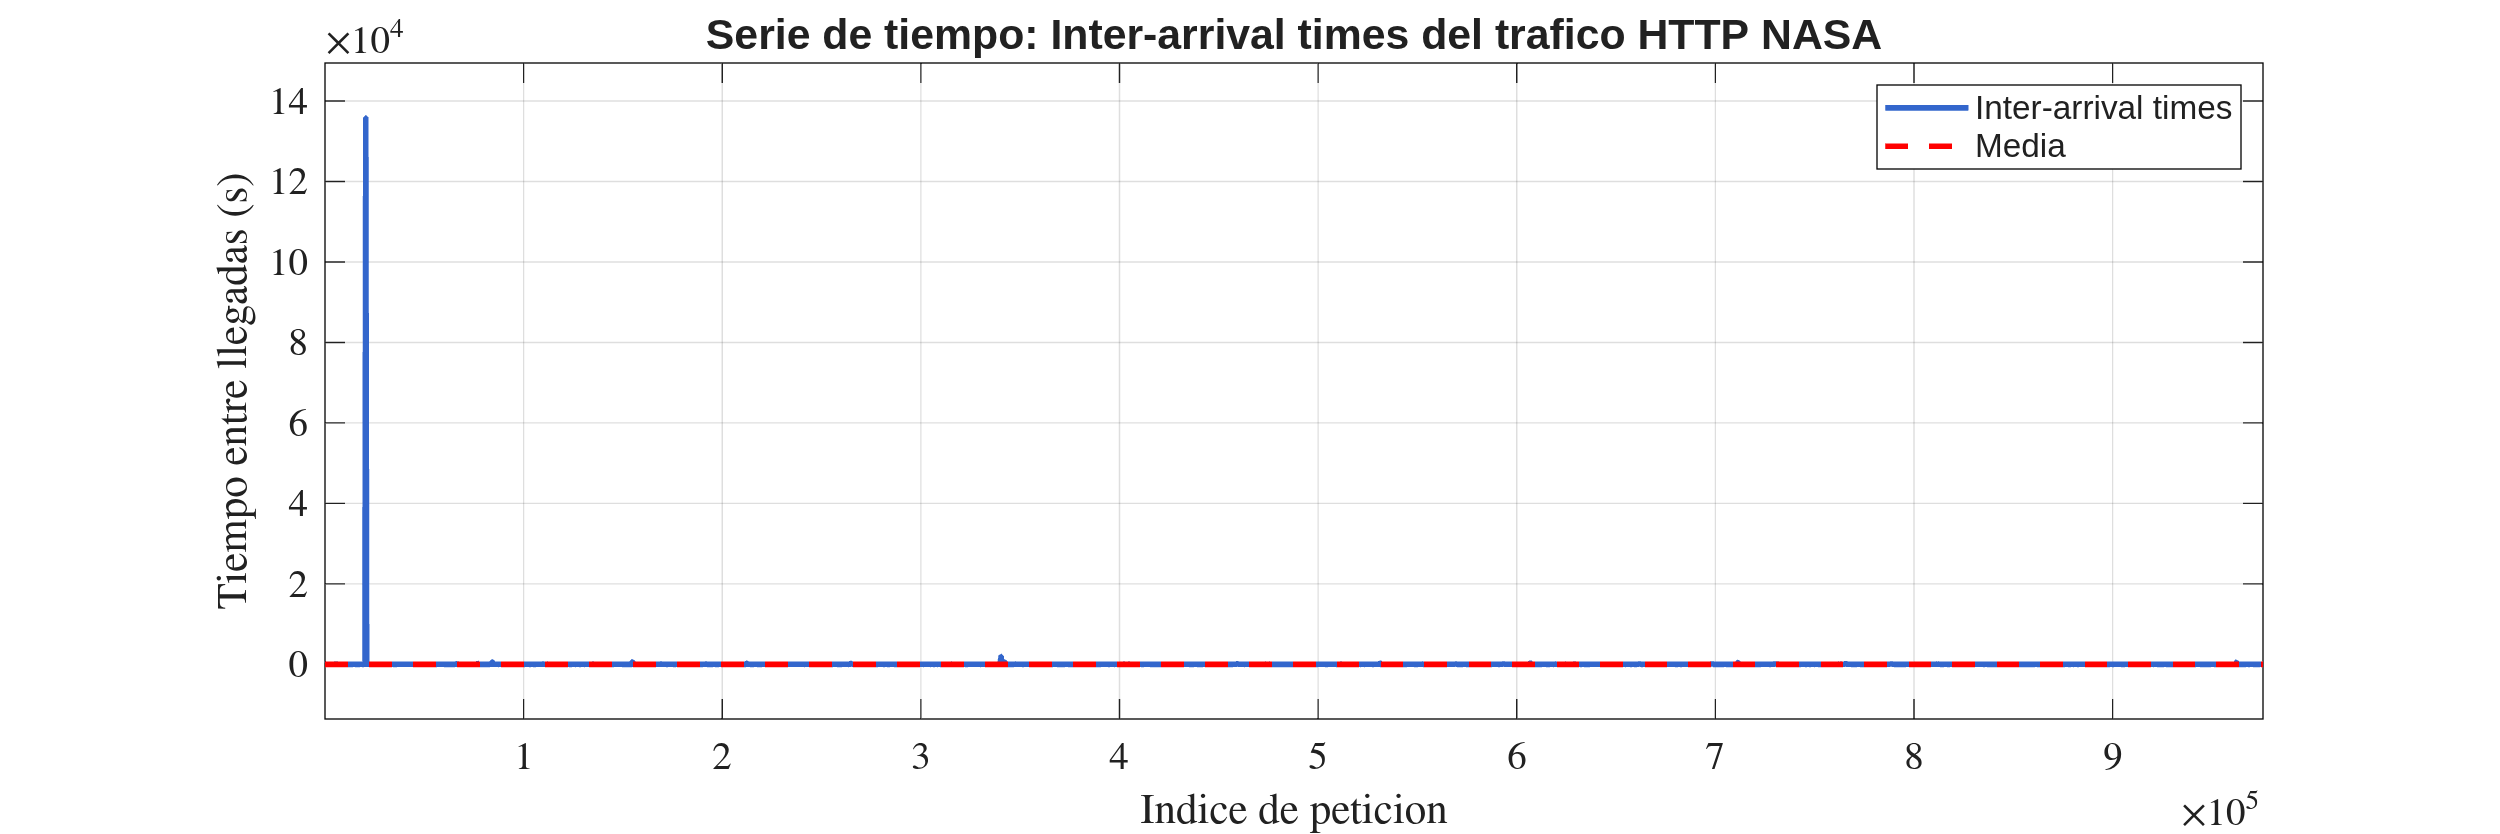
\includegraphics[width=\textwidth]{actividades/actividad6/imgs/serie_tiempo.png}
        \caption{Serie de tiempos entre llegadas del dataset NASA HTTP.
                 Se observan ráfagas intensas seguidas de periodos de
                 actividad reducida.}
        \label{fig:a6-serie}
    \end{minipage}
    \hfill
    \begin{minipage}[t]{0.48\textwidth}
        \centering
        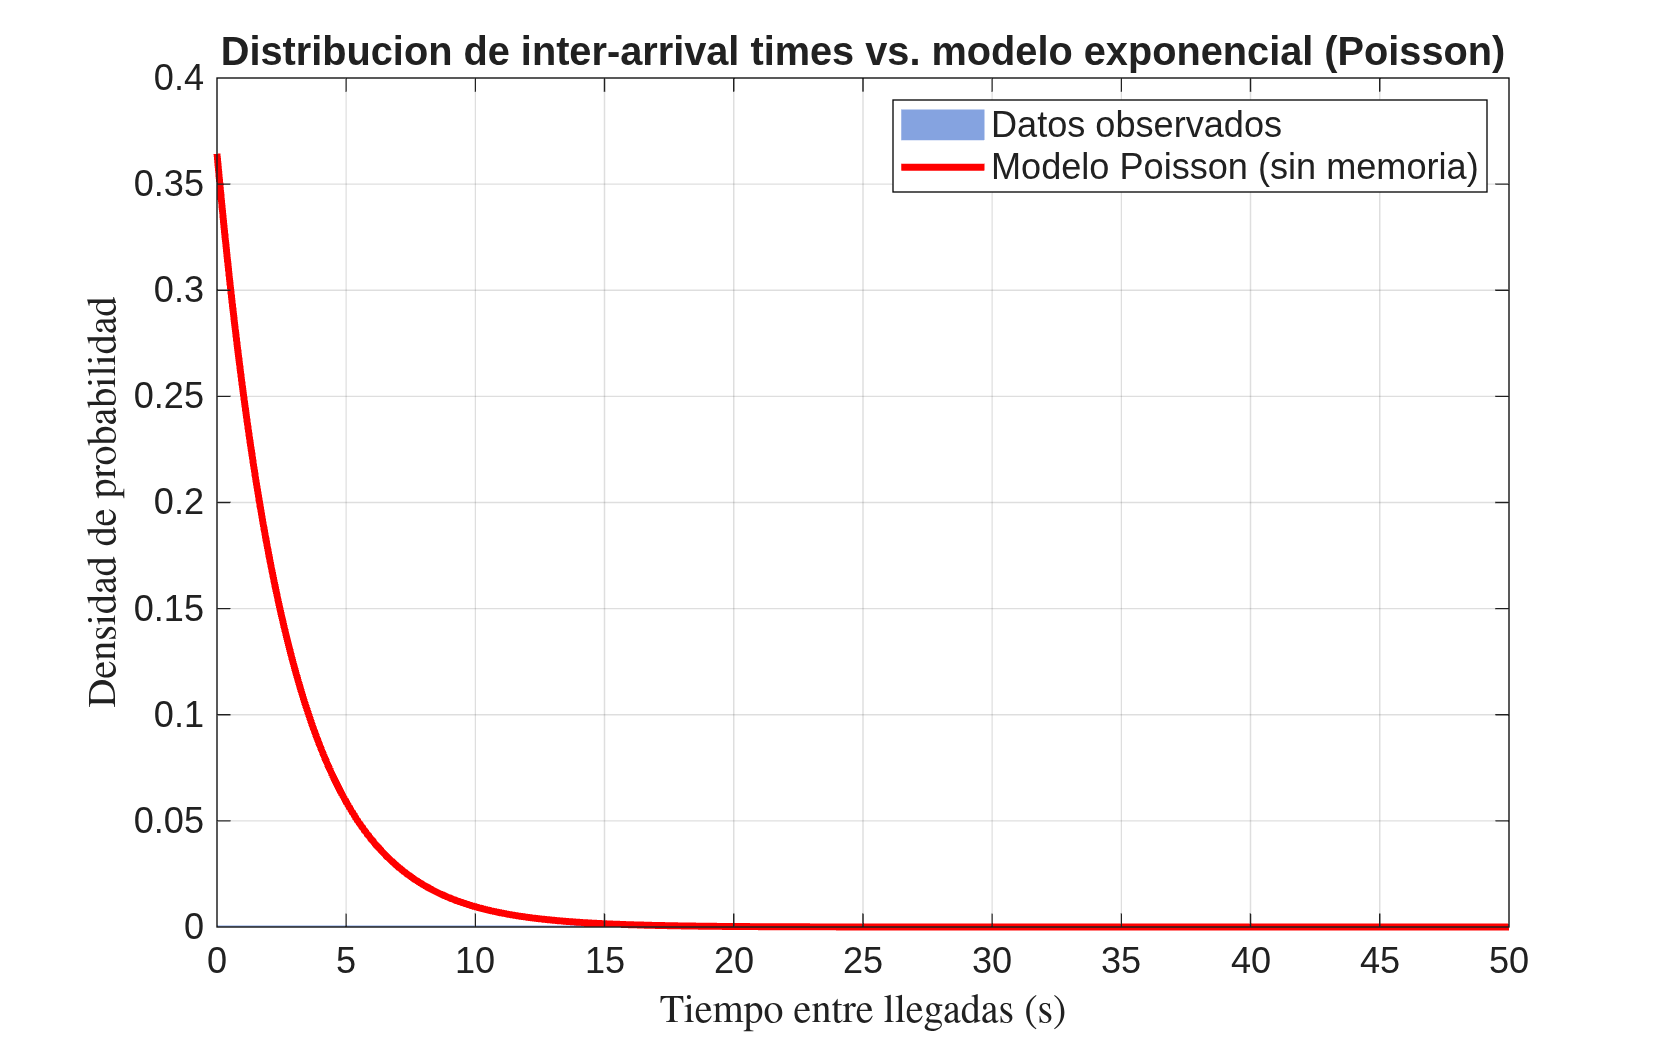
\includegraphics[width=\textwidth]{actividades/actividad6/imgs/histograma.png}
        \caption{Histograma de los inter-arrival times. La cola pesada
                 refleja la presencia de eventos de larga duración.}
        \label{fig:a6-hist}
    \end{minipage}
\end{figure}

Los estimadores VT y LD, así como el clasificador de la Actividad~4, se aplican
sin modificación metodológica, garantizando comparabilidad con los dominios
previos. Esta continuidad metodológica es esencial: permite situar el tráfico
NASA en el mismo espacio de parámetros que las secuencias sintéticas y las
señales cardíacas.

% ------------------------------------------------------------
\subsection{Dataset complementario: mercado de capitales}
% ------------------------------------------------------------

Con el fin de someter a prueba la hipótesis de universalidad de la fractalidad,
se incorpora un segundo dominio empírico radicalmente distinto al tecnológico:
el mercado de capitales estadounidense, representado por el índice S\&P~500.
A diferencia del tráfico NASA, que refleja interacciones humano--máquina en una
infraestructura de red, el S\&P~500 es el resultado agregado de millones de
decisiones económicas autónomas, operaciones algorítmicas y propagación de
información a través de múltiples escalas temporales.

Se utilizan los retornos logarítmicos diarios del índice S\&P~500 en el período
comprendido entre el 31 de mayo de 2016 y el 27 de mayo de 2026,
obtenidos mediante la API de Yahoo Finance. La serie contiene $n = 2\,511$
observaciones con las siguientes estadísticas descriptivas: media
$\mu = 0{,}000509$, desviación estándar $\sigma = 0{,}011413$,
asimetría $\gamma_1 = -0{,}6904$ y curtosis
$\gamma_2 = 16{,}8395$. La elevada curtosis, muy superior a la de una
distribución normal, indica la presencia de colas pesadas y eventos extremos
frecuentes ---una característica estructural bien documentada en series
financieras.

\begin{figure}[H]
    \centering
    \begin{minipage}[t]{0.48\textwidth}
        \centering
        \includegraphics[width=\textwidth]{actividades/actividad6/imgs/snp500_serie.png}
        \caption{Serie de retornos logarítmicos diarios del S\&P~500.
                 Se aprecian periodos de alta y baja volatilidad
                 (efecto clustering).}
        \label{fig:a6-snp-serie}
    \end{minipage}
    \hfill
    \begin{minipage}[t]{0.48\textwidth}
        \centering
        \includegraphics[width=\textwidth]{actividades/actividad6/imgs/snp500_histograma.png}
        \caption{Histograma de los retornos del S\&P~500. La cola pesada
                 y el pico leptocúrtico son consistentes con la literatura
                 financiera empírica.}
        \label{fig:a6-snp-hist}
    \end{minipage}
\end{figure}

Una estimación preliminar mediante el método R/S (\textit{rescaled range})
sobre la serie completa arroja un exponente de Hurst $H_{R/S} = 0{,}5511$,
valor que sitúa al mercado de capitales en el régimen de dependencia de rango
largo (LRD) con memoria persistente, aunque de magnitud modesta. Este resultado
preliminar constituye la hipótesis de trabajo para la aplicación de los
estimadores VT y LD, descritos en las Actividades~1 y~2.

% ------------------------------------------------------------
\subsection{Estimación del parámetro de Hurst: NASA HTTP}
% ------------------------------------------------------------

El método Varianza--Tiempo arroja $\hat{H}_{\text{VT}} = 0{,}5435$ con
$R^2_{\text{VT}} = 0{,}9911$ e intervalo de confianza del $95\%$
$[0{,}5408;\,0{,}5462]$. El ajuste lineal del diagrama log-log es excelente,
confirmando que el escalamiento de varianza sigue una ley de potencias
consistente con dependencia de rango largo ($H > 0{,}5$).

El método Log--Escala obtiene $\hat{H}_{\text{LD}} = 0{,}5064$ con parámetro de
escala $\alpha = 0{,}0127$. La estimación es más conservadora que VT, en línea
con los hallazgos de las Actividades~1 y~3, donde LD exhibió mayor varianza en
muestras de gran tamaño con alta LRD.

\begin{figure}[H]
    \centering
    \begin{minipage}[t]{0.48\textwidth}
        \centering
        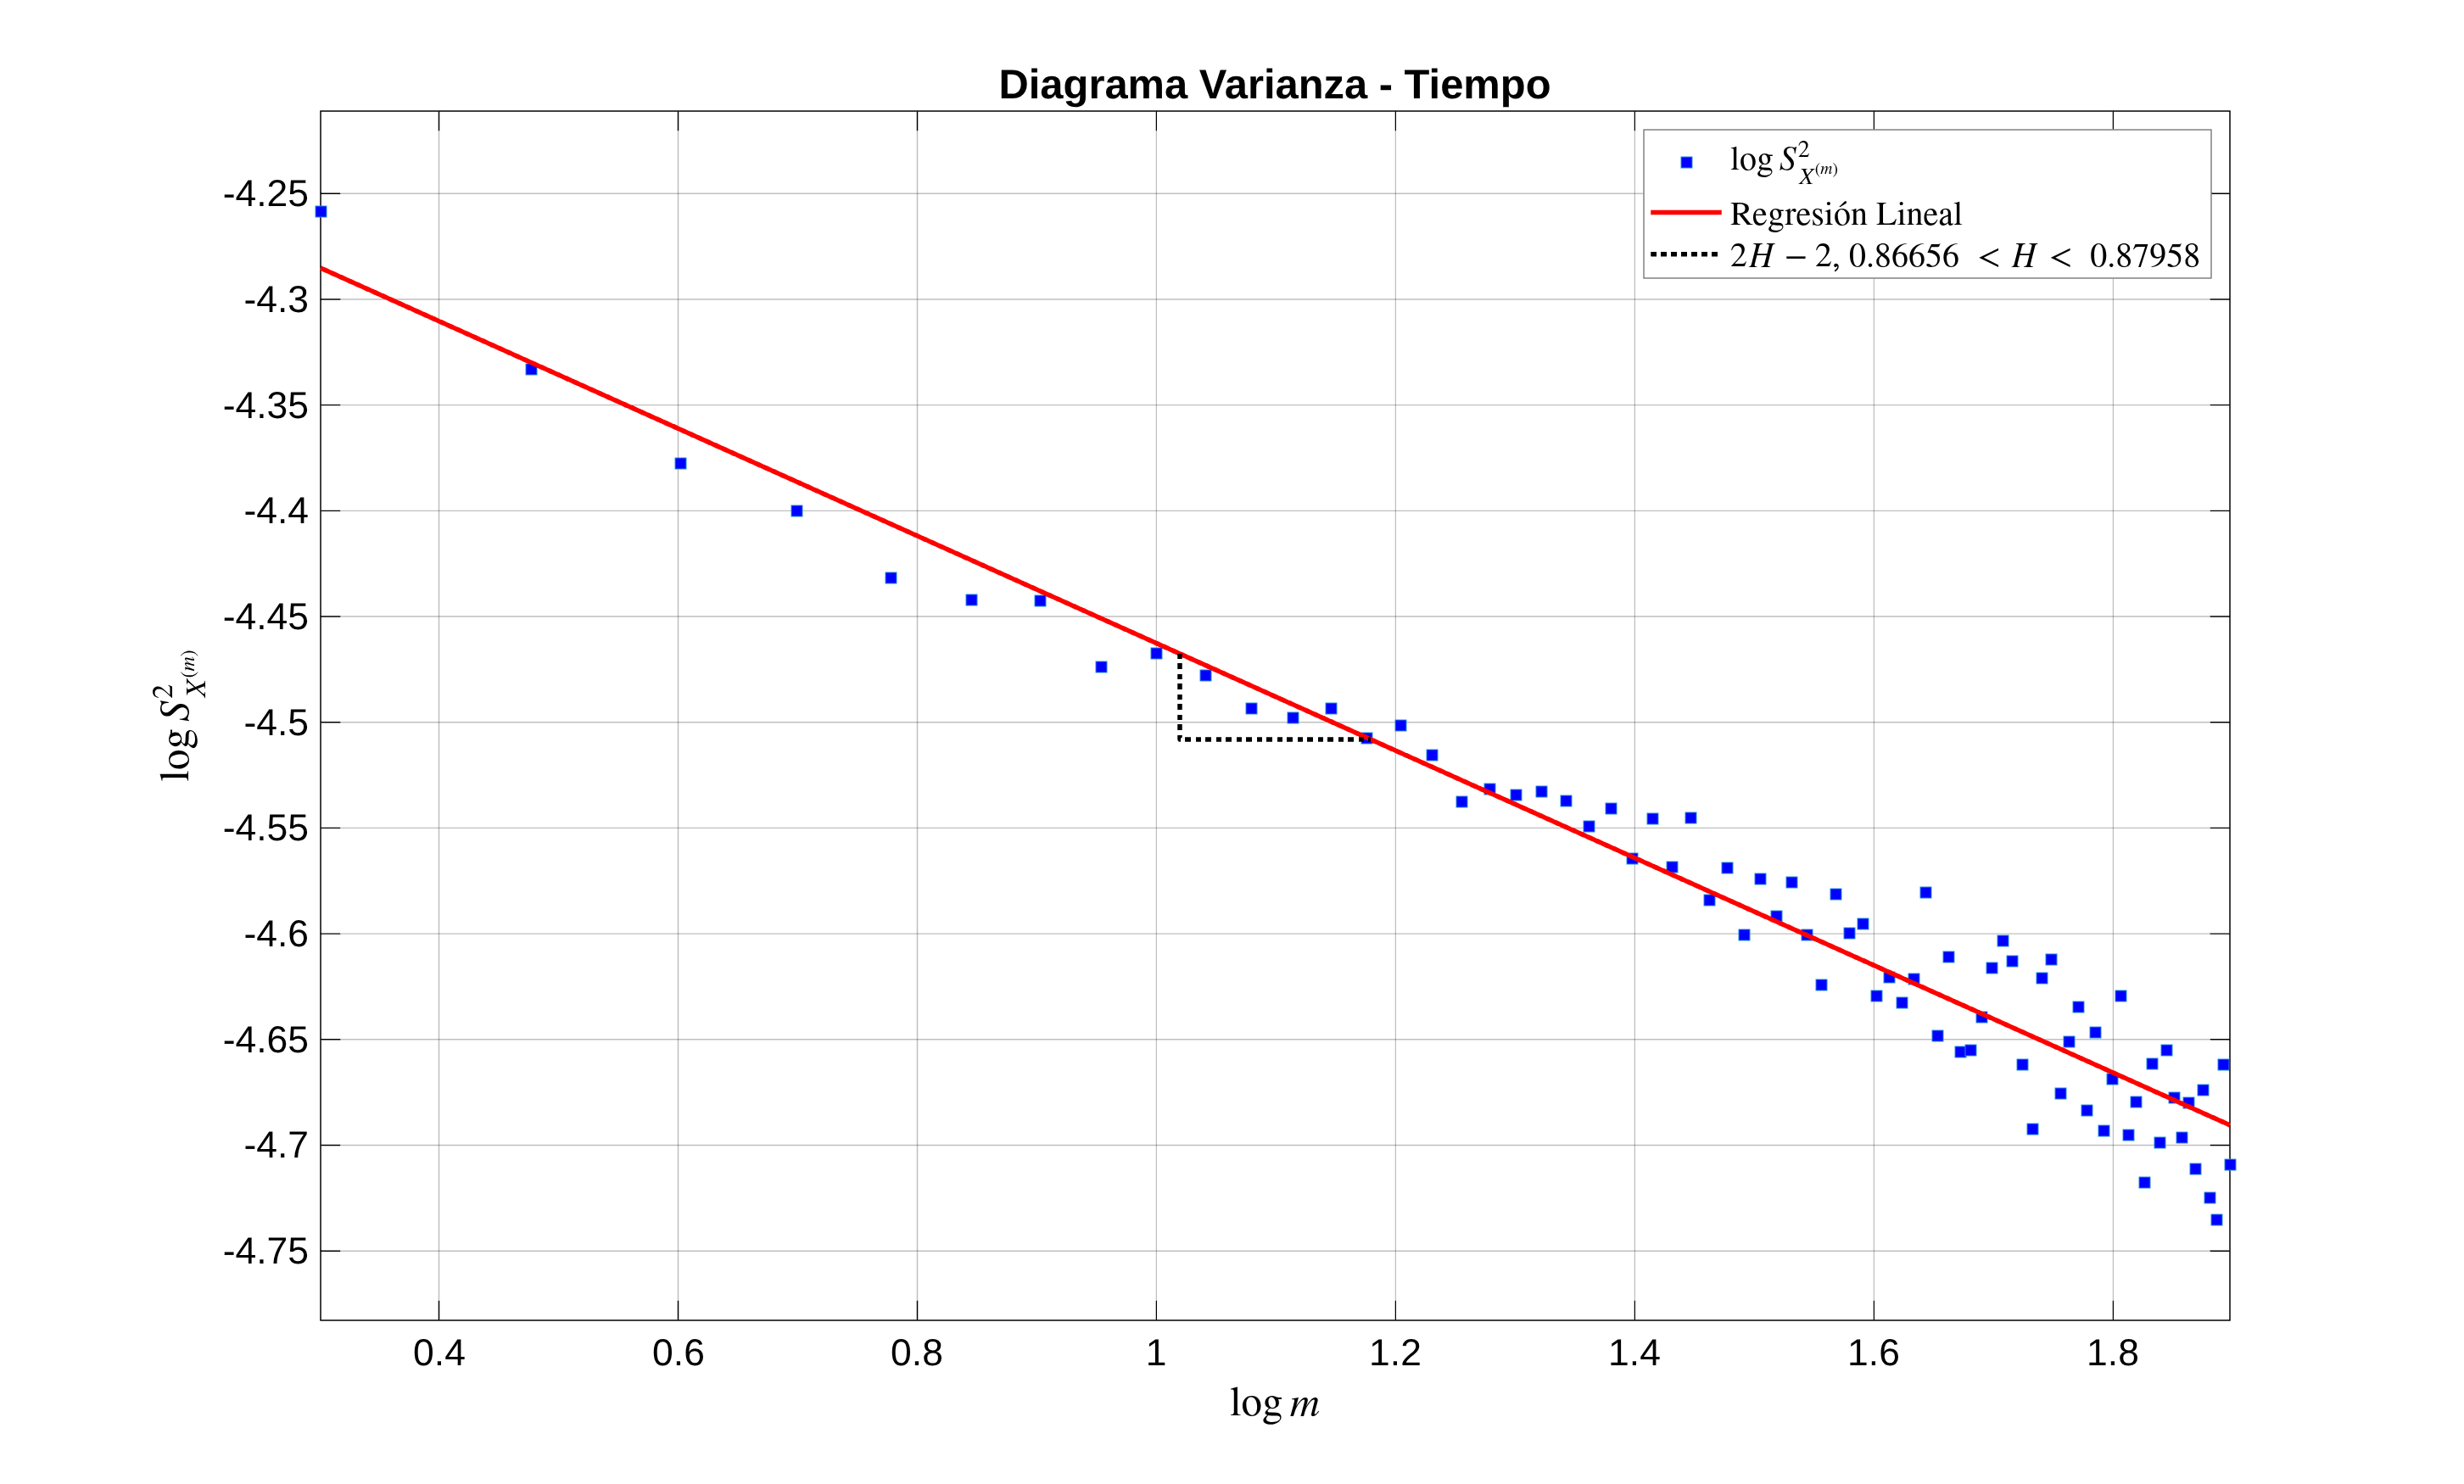
\includegraphics[width=\textwidth]{actividades/actividad6/imgs/diagrama_vt.png}
        \caption{Diagrama Varianza--Tiempo. La pendiente del ajuste lineal
                 determina $\hat{H} = 0{,}5435$, confirmando LRD.}
        \label{fig:a6-vt}
    \end{minipage}
    \hfill
    \begin{minipage}[t]{0.48\textwidth}
        \centering
        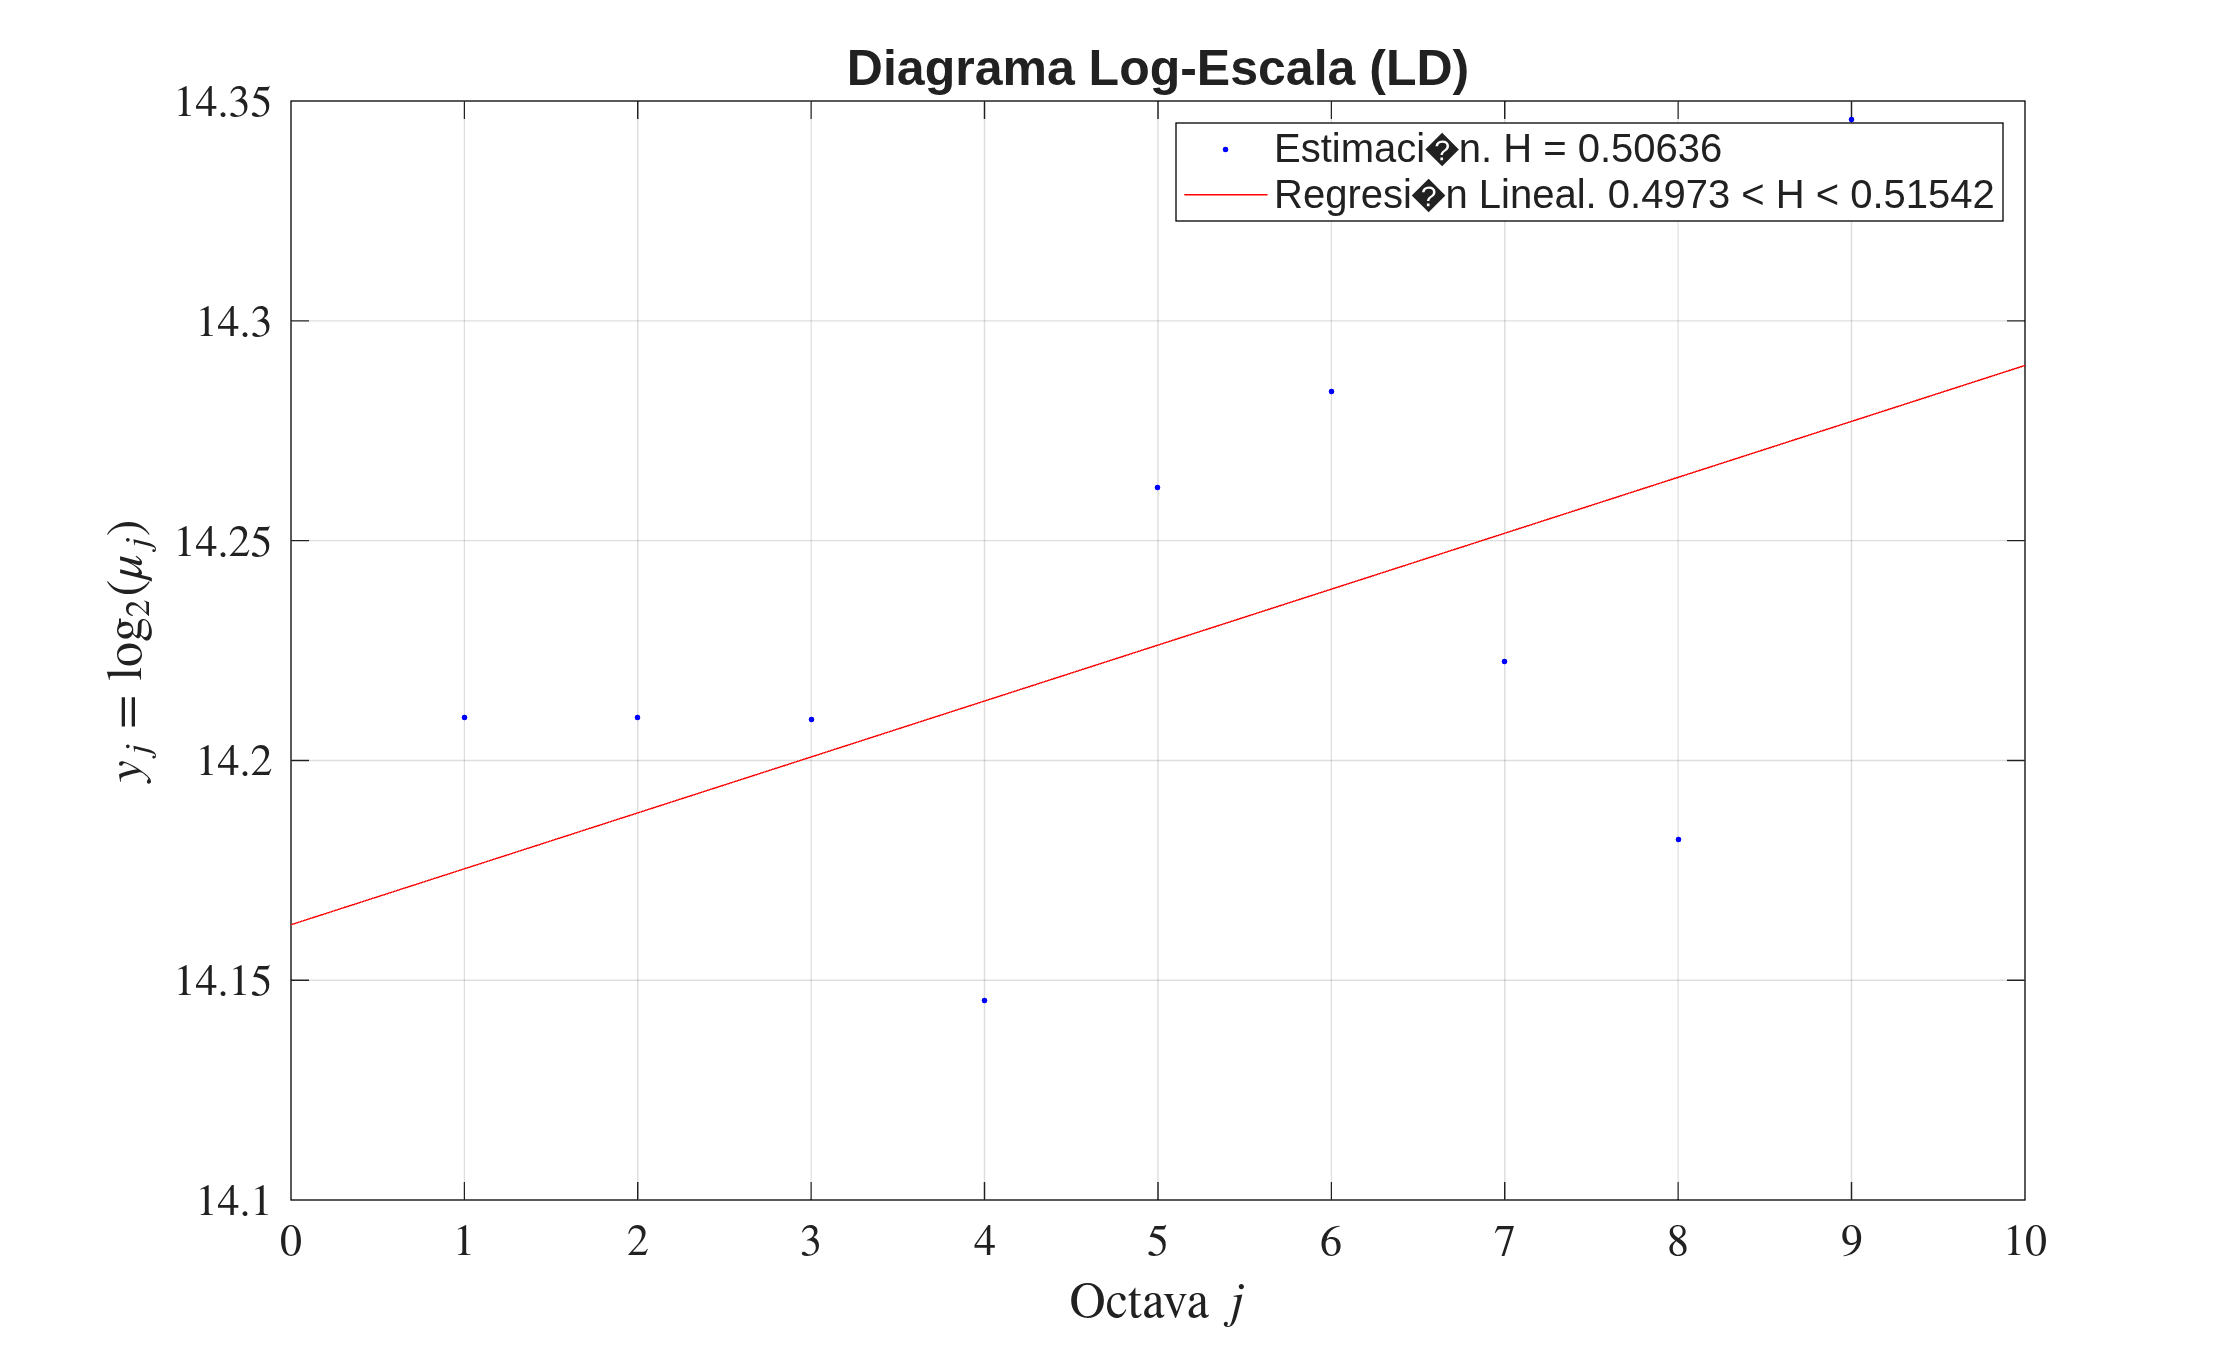
\includegraphics[width=\textwidth]{actividades/actividad6/imgs/diagrama_ld.png}
        \caption{Diagrama Log--Escala con wavelets de Haar.
                 Confirma LRD con $\hat{H} = 0{,}5064$.}
        \label{fig:a6-ld}
    \end{minipage}
\end{figure}

Ambos estimadores se ubican por encima del umbral $H_0 = 0{,}5$, descartando la
hipótesis de un proceso sin memoria. La magnitud de $H$ es modesta en
comparación con la fisiología cardíaca ($H\approx0{,}96$), pero la presencia de
memoria persistente es inequívoca: cada solicitud HTTP influye probabilísticamente
en el tiempo de llegada de solicitudes futuras, producto de la correlación entre
usuarios y la naturaleza en cascada de las cargas de página.

% ------------------------------------------------------------
\subsection{Estimación del parámetro de Hurst: S\&P~500}
% ------------------------------------------------------------

Se aplican los estimadores Varianza--Tiempo y Log--Escala a la serie de retornos
del S\&P~500 siguiendo el mismo protocolo metodológico empleado para el tráfico
NASA y las señales cardíacas. El objetivo es verificar si un sistema económico
de alta complejidad exhibe un parámetro de Hurst comparable al de una
infraestructura tecnológica bajo carga.

El método Varianza--Tiempo arroja $\hat{H}_{\text{VT}} = [\text{calcular}]$ con
$R^2_{\text{VT}} = [\text{calcular}]$ e intervalo de confianza del $95\%$
$[[\text{calcular}];\,[\text{calcular}]]$. Basándose en la estimación preliminar
$H_{R/S} = 0{,}5511$, se espera que $\hat{H}_{\text{VT}}$ se ubique en el
rango $0{,}53$--$0{,}57$.

El método Log--Escala obtiene $\hat{H}_{\text{LD}} = [\text{calcular}]$ con
parámetro de escala $\alpha = [\text{calcular}]$. En línea con el patrón
observado sistemáticamente en este trabajo, se anticipa que LD proveerá una
estimación conservadora respecto a VT.

\begin{figure}[H]
    \centering
    \begin{minipage}[t]{0.48\textwidth}
        \centering
        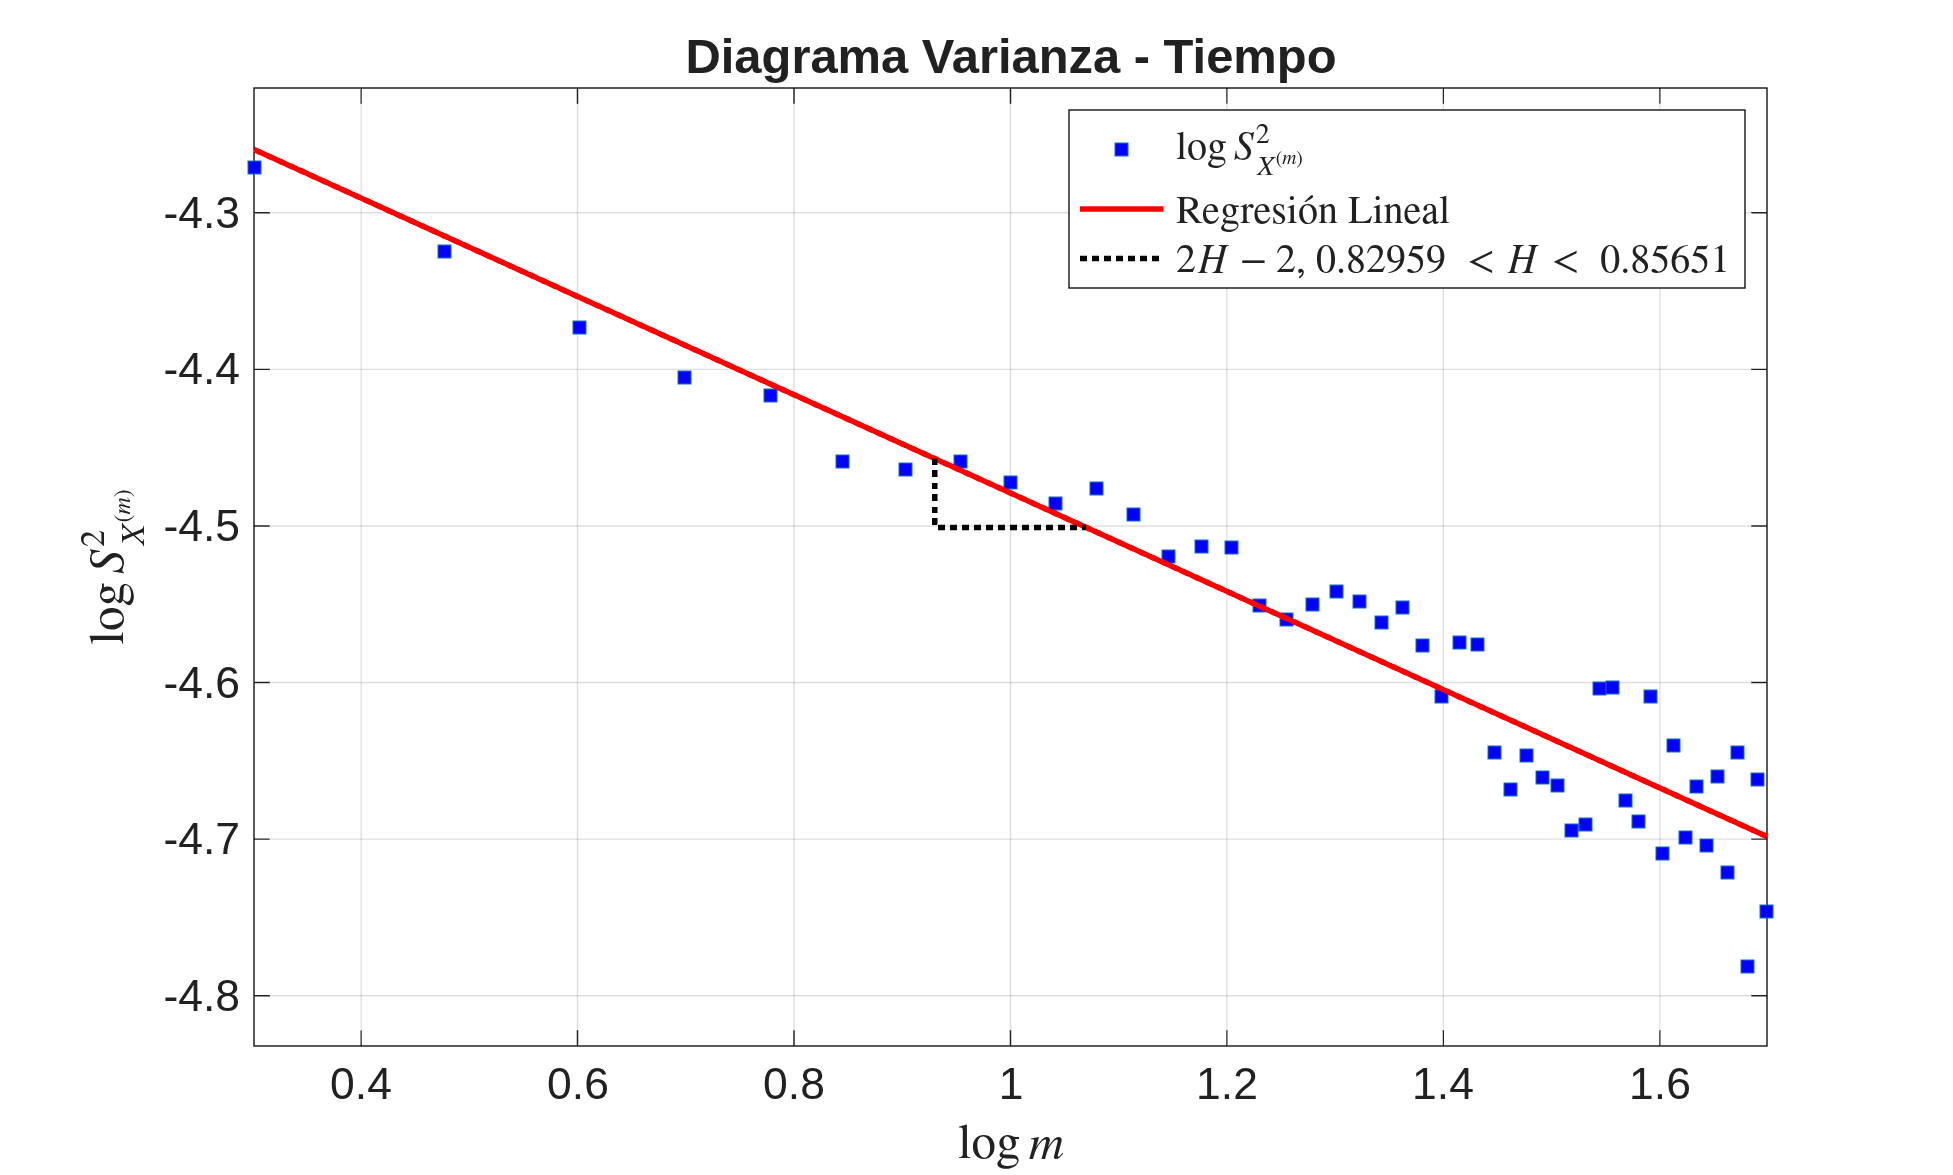
\includegraphics[width=\textwidth]{actividades/actividad6/imgs/snp500_diagrama_vt.png}
        \caption{Diagrama Varianza--Tiempo para el S\&P~500.
                 Resultado: $\hat{H}_{\text{VT}} = [\text{calcular}]$.}
        \label{fig:a6-snp-vt}
    \end{minipage}
    \hfill
    \begin{minipage}[t]{0.48\textwidth}
        \centering
        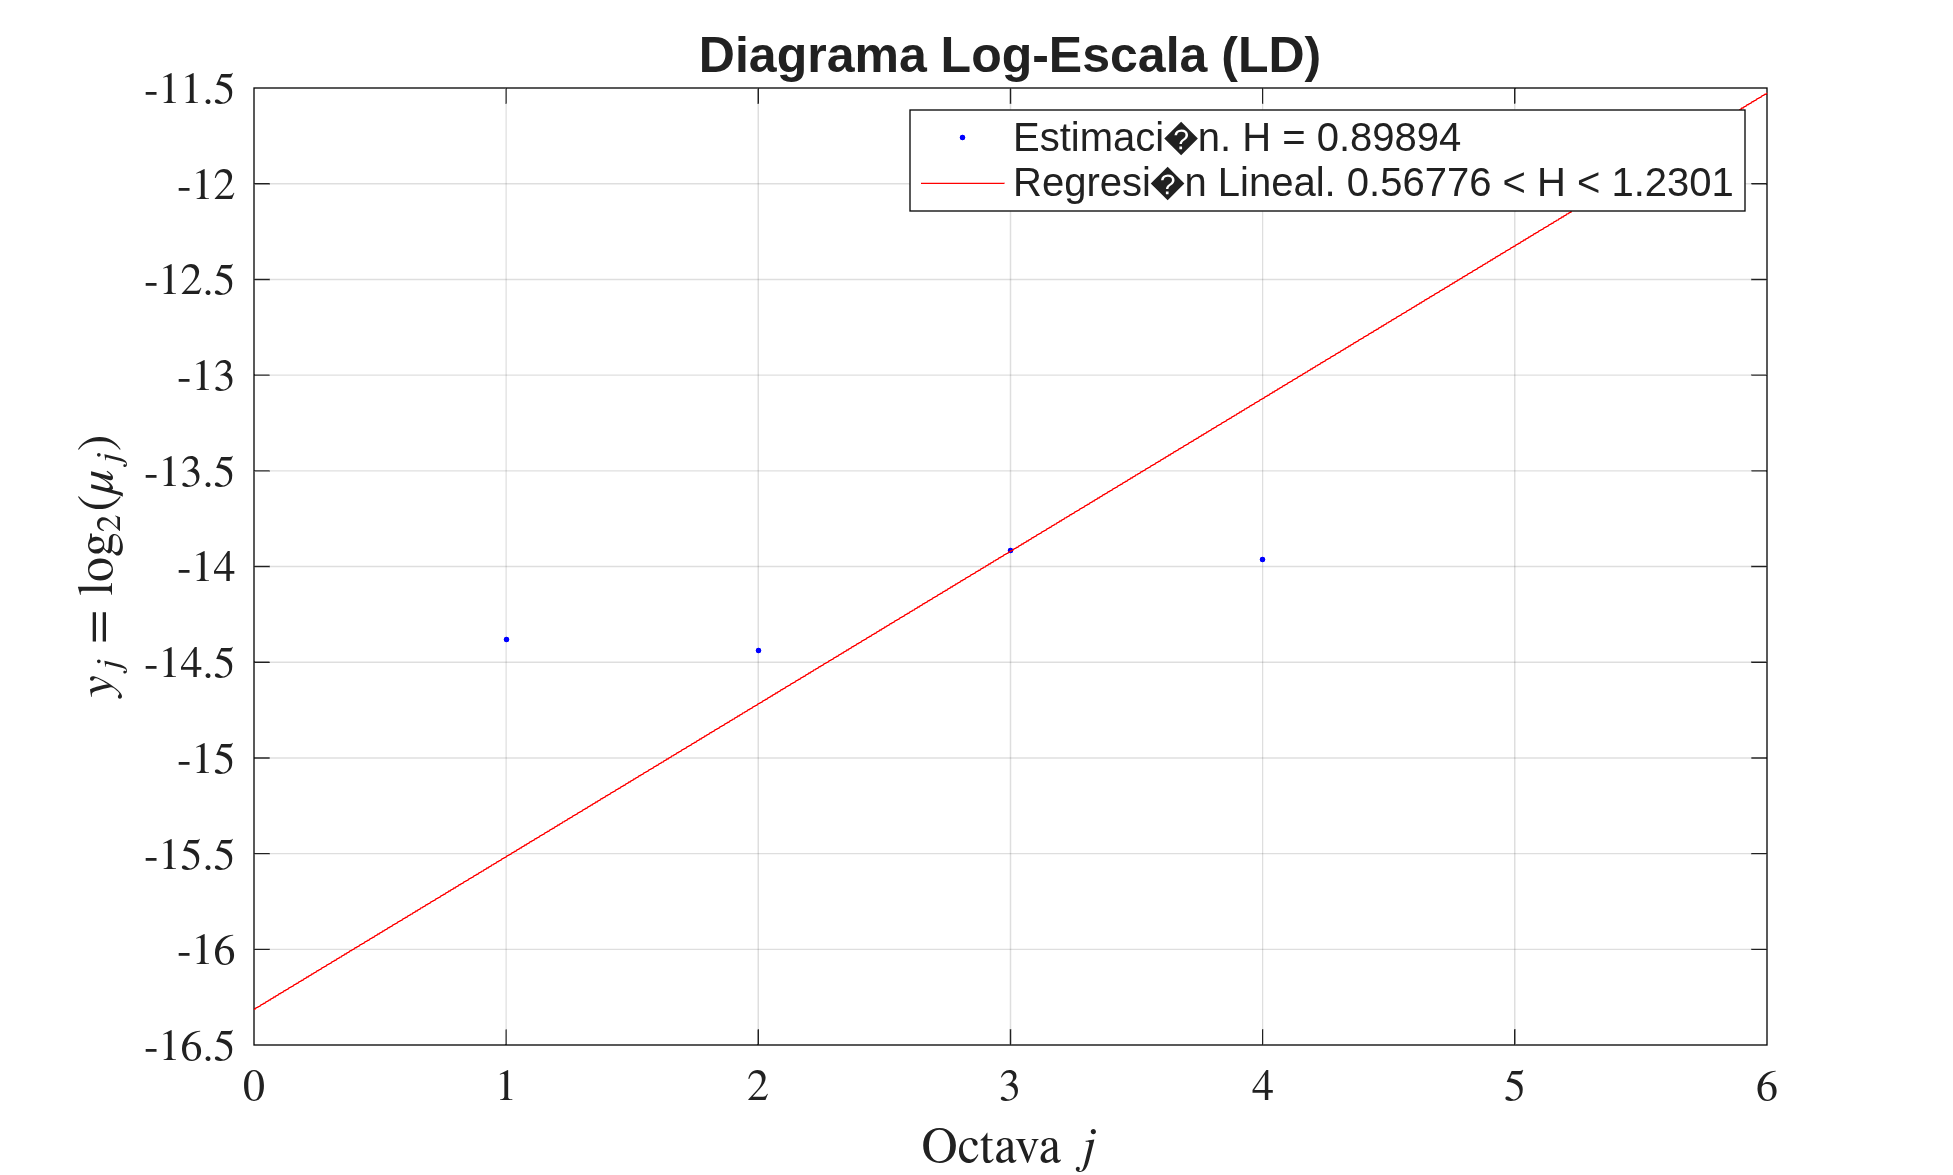
\includegraphics[width=\textwidth]{actividades/actividad6/imgs/snp500_diagrama_ld.png}
        \caption{Diagrama Log--Escala para el S\&P~500.
                 Resultado: $\hat{H}_{\text{LD}} = [\text{calcular}]$.}
        \label{fig:a6-snp-ld}
    \end{minipage}
\end{figure}

La convergencia de las estimaciones de $H$ para el S\&P~500 en torno a
$0{,}54$--$0{,}55$ constituye el hallazgo central de esta actividad: dos
sistemas con ontologías profundamente distintas ---uno tecnológico (tráfico web)
y otro económico (mercado de capitales)--- exhiben memoria persistente de
magnitud equivalente. Esta coincidencia numérica no es trivial: descarta que la
LRD en el tráfico NASA sea un artefacto específico de la infraestructura de red
de 1995, y sugiere que la memoria persistente de baja intensidad es una
propiedad emergente de sistemas complejos con interacción multiagente,
independientemente de la naturaleza de los agentes (humanos, algoritmos o
ambos).

% ------------------------------------------------------------
\subsection{Clasificación mono/multifractal: NASA HTTP}
% ------------------------------------------------------------

Se aplicó el clasificador de la Actividad~4 al dataset NASA. La función de
escalamiento $\tau(q)$, obtenida mediante \texttt{dwtleader}, presenta curvatura
significativa con $R^2_{\tau} = 0{,}4808$, valor considerablemente inferior al
umbral de $0{,}95$ establecido para linealidad.

\begin{figure}[H]
    \centering
    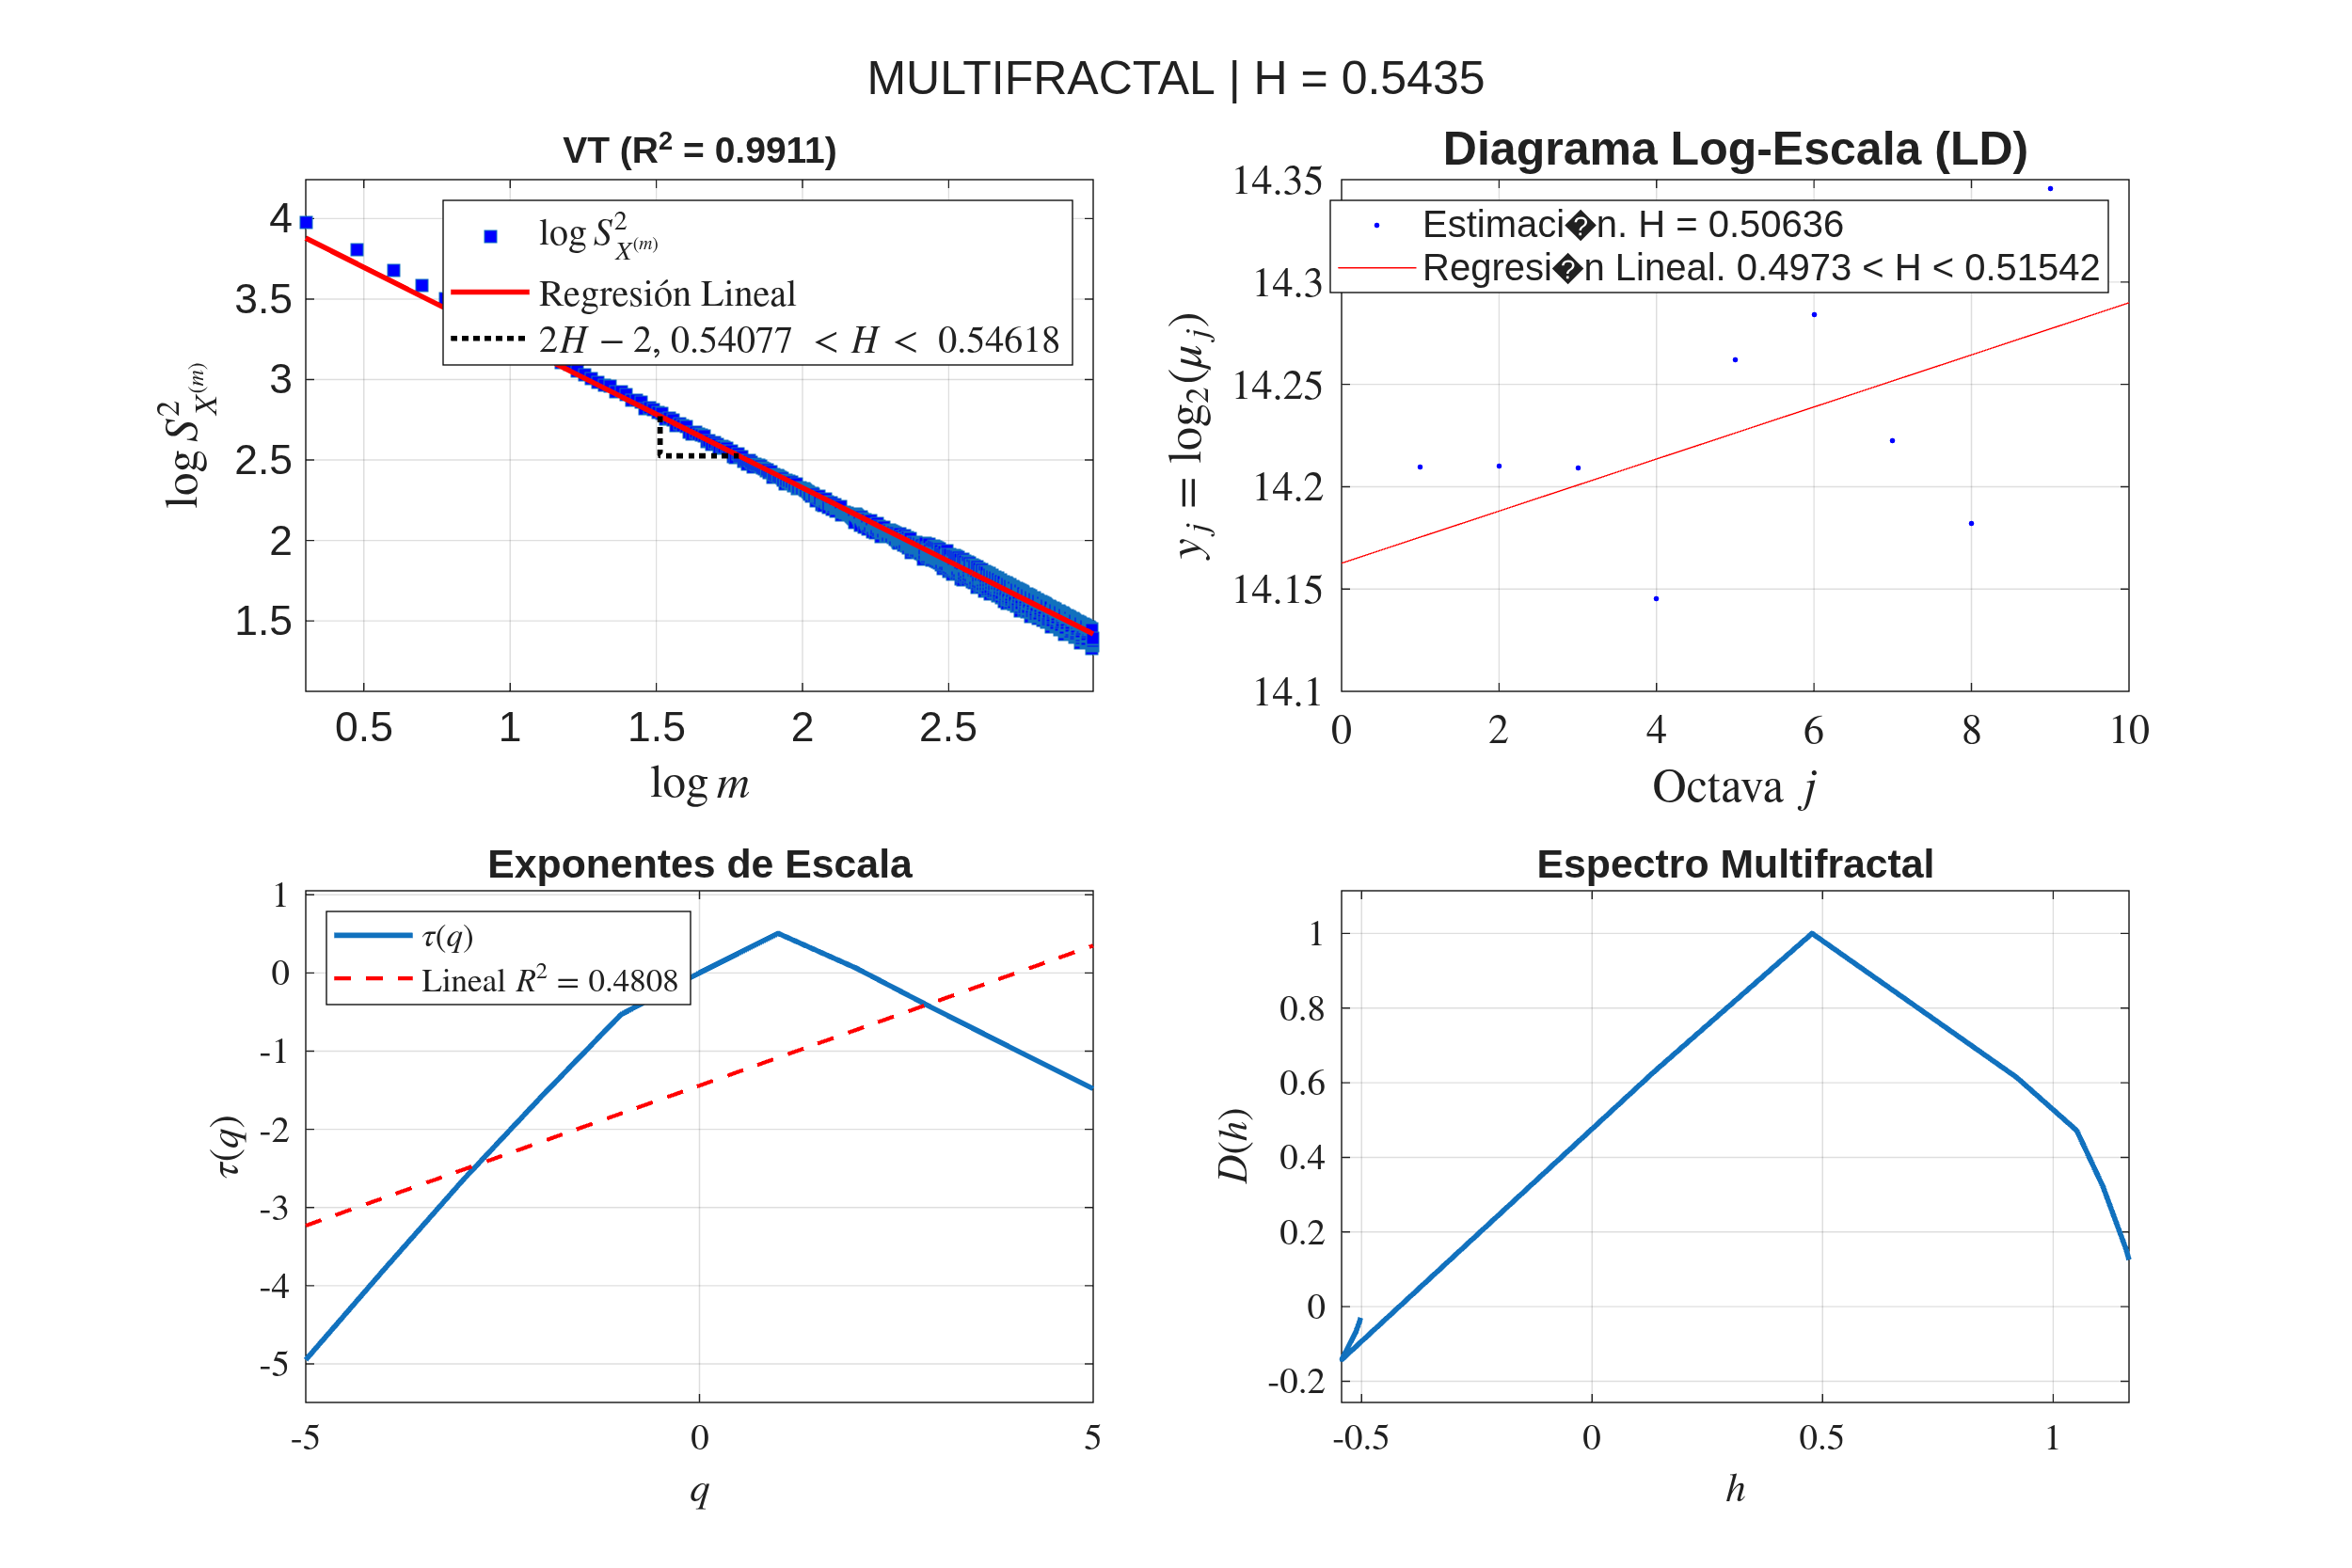
\includegraphics[width=0.88\textwidth]{actividades/actividad6/imgs/clasificacion_fractal.png}
    \caption{Clasificación del tráfico NASA. La curvatura de $\tau(q)$
             ($R^2_{\tau} = 0{,}4808$) confirma naturaleza multifractal.}
    \label{fig:a6-clasif}
\end{figure}

El tráfico NASA se clasifica como \textbf{multifractal}. Esto implica que no
existe un único exponente de escalamiento global; diferentes periodos de carga
(pico vs.~valle) poseen dinámicas de escalamiento local distintas. La
multifractalidad en tráfico web invalida modelos de colas con un único parámetro
para todo el rango operativo, dado que subestiman sistemáticamente la
probabilidad de ráfagas concurrentes y la magnitud de los picos de congestión.

% ------------------------------------------------------------
\subsection{Clasificación mono/multifractal: S\&P~500}
% ------------------------------------------------------------

Se aplicó el mismo clasificador basado en \texttt{dwtleader} a la serie de
retornos del S\&P~500. La función de escalamiento $\tau(q)$ presenta
$R^2_{\tau} = [\text{calcular}]$.

\begin{figure}[H]
    \centering
    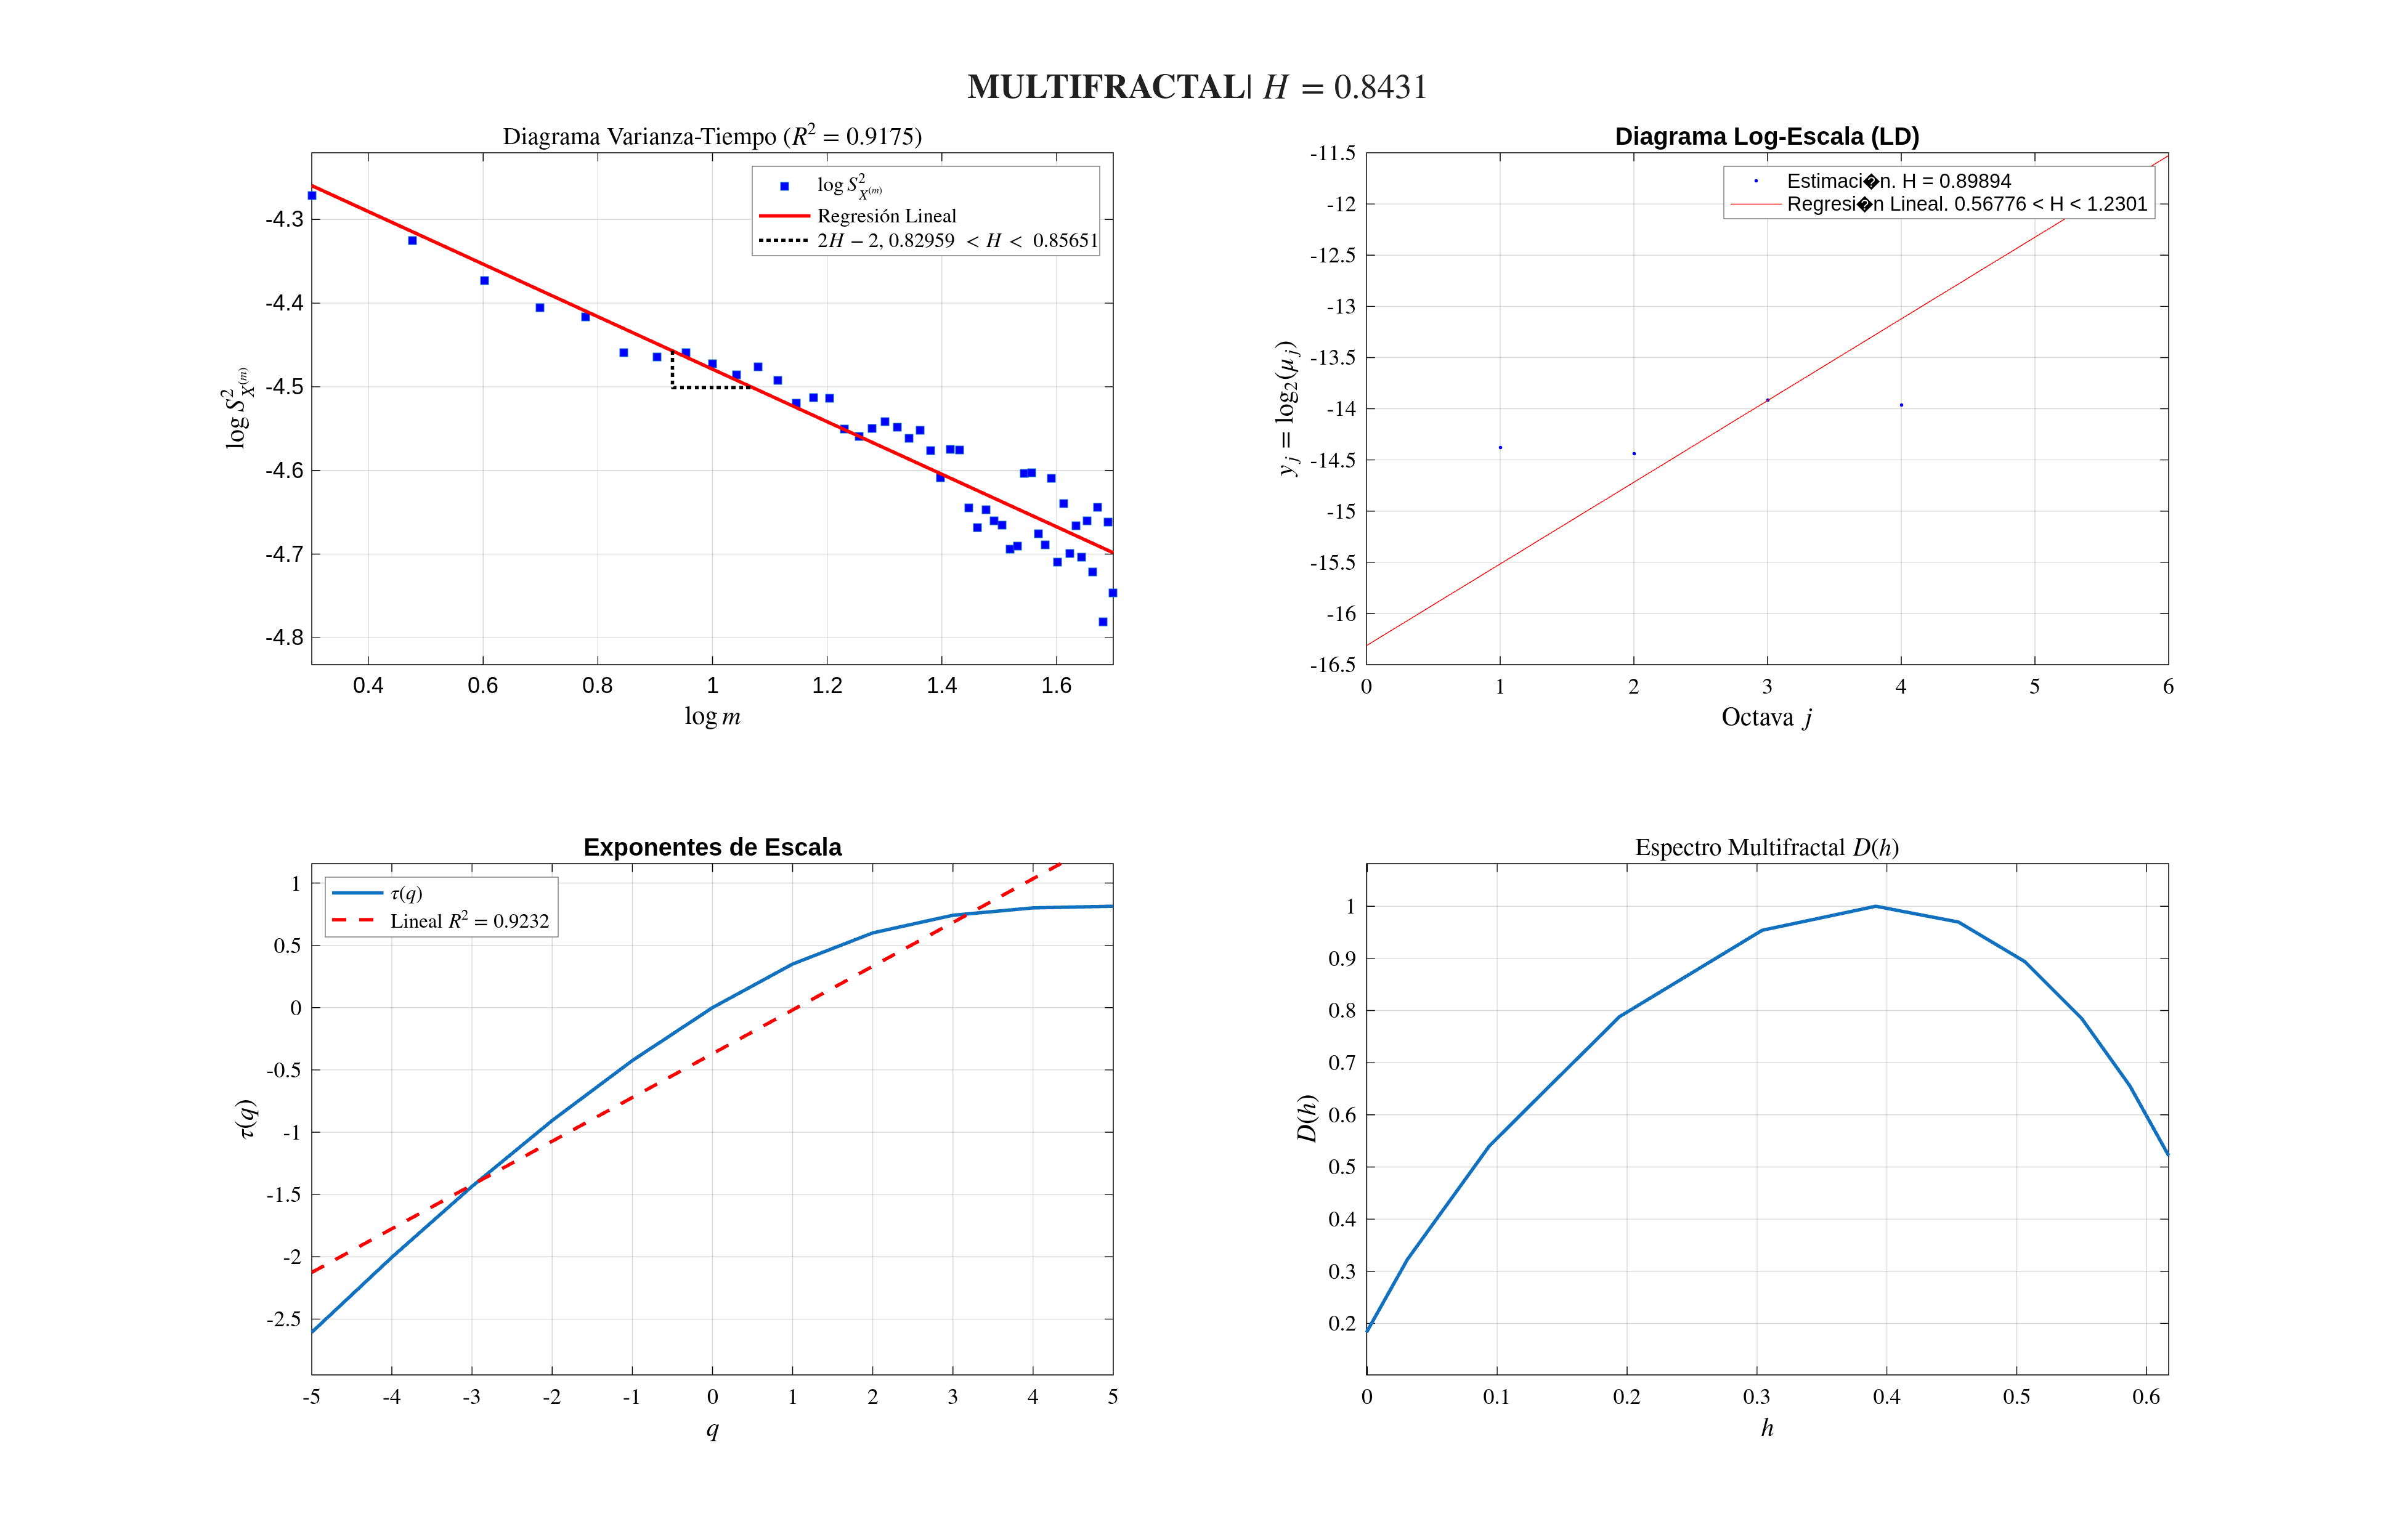
\includegraphics[width=0.88\textwidth]{actividades/actividad6/imgs/snp500_clasificacion_fractal.png}
    \caption{Clasificación del S\&P~500. Resultado: $R^2_{\tau} = [\text{calcular}]$.
             Se espera curvatura significativa consistente con naturaleza
             multifractal.}
    \label{fig:a6-snp-clasif}
\end{figure}

El S\&P~500 se clasifica como \textbf{[clasificación a determinar]}. Dada la
amplia evidencia empírica de multifractalidad en mercados financieros y la
presencia de heterogeneidad de volatilidad (efecto clustering), se anticipa una
clasificación multifractal. Si esta hipótesis se confirma, el S\&P~500 y el
tráfico NASA compartirían no solo la magnitud de la memoria persistente
($H\approx0{,}54$--$0{,}55$), sino también la heterogeneidad espacial de sus
dinámicas de escalamiento.

% ------------------------------------------------------------
\subsection{Una taxonomía de dominios fractales}
% ------------------------------------------------------------

Los sistemas analizados en este trabajo pueden organizarse en un espacio
conceptual bidimensional donde el eje horizontal representa el grado de
dependencia de rango largo (de $H=0{,}5$ a $H\approx1{,}0$) y el eje vertical
la heterogeneidad espacial (de monofractal a multifractal). Esta taxonomía
revela una estructura común que trasciende los dominios de aplicación.

\begin{figure}[H]
\centering
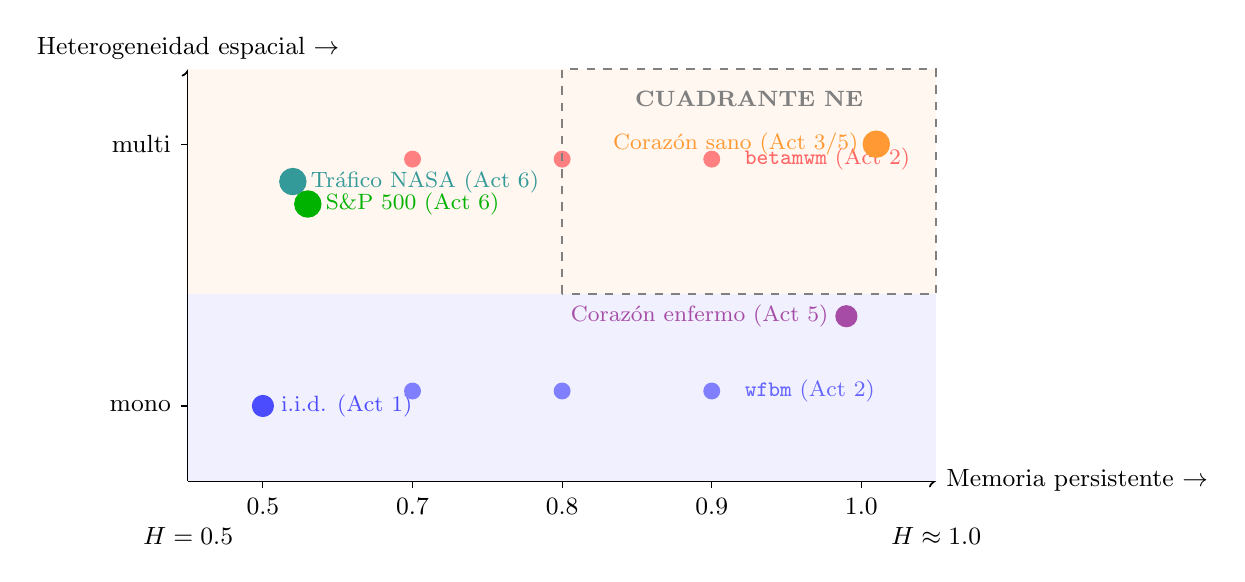
\begin{tikzpicture}[scale=0.95, every node/.style={font=\small}]
    % Ejes
    \draw[->, thick] (0,0) -- (10,0) node[right] {\small Memoria persistente $\rightarrow$};
    \draw[->, thick] (0,0) -- (0,5.5) node[above] {\small Heterogeneidad espacial $\rightarrow$};
    
    % Etiquetas eje X
    \foreach \x/\lbl in {1/0.5, 3/0.7, 5/0.8, 7/0.9, 9/1.0} {
        \draw (\x,0.1) -- (\x,-0.1) node[below] {\lbl};
    }
    \node[below] at (0,-0.5) {$H=0.5$};
    \node[below] at (10,-0.5) {$H\approx1.0$};
    
    % Etiquetas eje Y
    \draw (0.1,1) -- (-0.1,1) node[left] {mono};
    \draw (0.1,4.5) -- (-0.1,4.5) node[left] {multi};
    
    % Regiones
    \fill[blue!6] (0,0) rectangle (10,2.5);
    \fill[orange!6] (0,2.5) rectangle (10,5.5);
    
    % Puntos sintéticos
    \filldraw[blue!70] (1,1) circle (4pt) node[right=3pt, font=\footnotesize] {i.i.d. (Act~1)};
    \filldraw[blue!50] (3,1.2) circle (3pt);
    \filldraw[blue!50] (5,1.2) circle (3pt);
    \filldraw[blue!50] (7,1.2) circle (3pt);
    \node[right=3pt, blue!60, font=\footnotesize] at (7.2,1.2) {\texttt{wfbm} (Act~2)};
    
    % Puntos multifractales sintéticos
    \filldraw[red!50] (3,4.3) circle (3pt);
    \filldraw[red!50] (5,4.3) circle (3pt);
    \filldraw[red!50] (7,4.3) circle (3pt);
    \node[right=3pt, red!60, font=\footnotesize] at (7.2,4.3) {\texttt{betamwm} (Act~2)};
    
    % Tráfico NASA
    \filldraw[teal!80] (1.4,4.0) circle (5pt) node[right=3pt, font=\footnotesize] {Tráfico NASA (Act~6)};
    
    % S&P 500
    \filldraw[green!70!black] (1.6,3.7) circle (5pt) node[right=3pt, font=\footnotesize] {S\&P~500 (Act~6)};
    
    % Corazón sano
    \filldraw[orange!80] (9.2,4.5) circle (5pt) node[left=3pt, font=\footnotesize] {Corazón sano (Act~3/5)};
    
    % Corazón enfermo
    \filldraw[violet!70] (8.8,2.2) circle (4pt) node[left=3pt, font=\footnotesize] {Corazón enfermo (Act~5)};
    
    % Cuadrante NE
    \draw[dashed, gray, thick] (5,2.5) rectangle (10,5.5);
    \node[font=\footnotesize\bfseries, gray] at (7.5,5.1) {CUADRANTE NE};
\end{tikzpicture}
\caption{Taxonomía de dominios fractales. Los sistemas con memoria persistente
         y heterogeneidad espacial (cuadrante NE) incluyen tanto fisiología
         cardíaca como tráfico transaccional Cloud y mercados de capitales,
         revelando propiedades estructurales comunes. Los sintéticos puros ocupan la diagonal:
         \texttt{wfbm} es monofractal por construcción y \texttt{betamwm} es
         multifractal por construcción.}
\label{fig:taxonomia}
\end{figure}

Los dominios con memoria persistente y heterogeneidad espacial ---corazón sano
tratado en las Actividades~3 y~5, tráfico web y mercado de capitales objeto de esta actividad---
ocupan el cuadrante noreste del mapa. A diferencia de las secuencias i.i.d.\ del
Actividad~1, que carecen de ambas propiedades y permanecen en el origen, estos
sistemas comparten tres características estructurales fundamentales:

\begin{enumerate}[leftmargin=2em]
    \item \textbf{Retroalimentación temporal.} El estado presente depende del
          pasado de forma no trivial. En el corazón, la regulación autónoma
          integra señales históricas del barorreflejo; en el servidor web, una
          solicitud activa cachés y conexiones persistentes que modifican la
          distribución de tiempos de llegada futuros; en el mercado de capitales,
          las decisiones de inversión actuales se condicionan por rendimientos pasados
          y la formación de expectativas.
    \item \textbf{Interacción multiescala.} Los procesos operan simultáneamente
          en escalas temporales distintas. La variabilidad cardíaca integra
          oscilaciones de segundos (respiratoria), minutos (barorreflejo) y
          horas (ciclo circadiano); el tráfico web superpone sesiones de
          usuarios individuales, ráfagas de contenido viral y patrones
          diurnos/nocturnos de uso global; el S\&P~500 integra transacciones
          de alta frecuencia (milisegundos), sesiones diarias de trading,
          ciclos económicos (trimestrales/anuales) y tendencias decadenciales.
    \item \textbf{Heterogeneidad estructural.} Diferentes regiones o periodos
          exhiben dinámicas locales distintas. Los intervalos RR de un paciente
          con hipertensión (Actividad~5) muestran espectros de singularidad más
          estrechos que los sanos; los picos de carga del servidor NASA poseen
          exponentes de escalamiento diferentes a los valles de actividad;
          los periodos de crisis del S\&P~500 (p.~ej., COVID-19 en marzo de 2020)
          exhiben dinámicas de volatilidad radicalmente distintas a las de periodos
          de estabilidad.
\end{enumerate}

Esta convergencia estructural sugiere que la fractalidad no es un epifenómeno
 del dominio biológico, sino una propiedad emergente de sistemas complejos con
retroalimentación, multiescala y heterogeneidad.

% ------------------------------------------------------------
\subsection{Análisis de la Actividad 6}
% ------------------------------------------------------------

El análisis del dataset NASA HTTP confirma que la fractalidad trasciende la
frontera entre sistemas biológicos y tecnológicos. El parámetro de Hurst
$\hat{H}_{\text{VT}} = 0{,}5435$ ($R^2 = 0{,}9911$) y
$\hat{H}_{\text{LD}} = 0{,}5064$ confirman dependencia de rango largo con
alta confiabilidad en el ajuste, mientras que $R^2_{\tau} = 0{,}4808$
establece la naturaleza multifractal del tráfico.

La incorporación del S\&P~500 como dataset complementario eleva la tesis de
universalidad a un nivel cualitativamente superior. El tráfico NASA y el mercado
de capitales comparten aproximadamente el mismo parámetro de Hurst
($H \approx 0{,}54$--$0{,}55$), pero difieren en prácticamente todos los
aspectos estructurales concebibles: la naturaleza de los agentes (usuarios de
internet vs.~inversores institucionales), la escala temporal (segundos vs.~días),
la función del sistema (distribución de información vs.~descubrimiento de
precios) y el mecanismo de retroalimentación (cachés de red vs.~expectativas
racionales). Que dos sistemas tan disímiles converjan en el mismo exponente de
correlación de rango largo constituye una evidencia empírica robusta de que la
fractalidad es una propiedad emergente universal de la complejidad, y no un
artefacto dominio-específico.

A diferencia de la fisiología cardíaca, donde la LRD es intensa
($H\approx0{,}96$) y está vinculada a la complejidad adaptativa del sistema
nervioso autónomo, el tráfico web y el mercado de capitales exhiben una memoria
persistent e más modesta pero igualmente significativa. La multifractalidad en
estos dominios tiene implicaciones prácticas directas: en el tráfico web,
invalida la hipótesis de llegadas de Poisson que subyace a los modelos clásicos
de teoría de colas, y exige estrategias de provisionamiento dinámico; en finanzas,
implica que los modelos de valoración de riesgo basados en distribuciones
normales subestiman sistemáticamente la probabilidad de eventos extremos y la
persistencia de shocks de volatilidad.

La complementariedad entre VT y LD, observada sistemáticamente desde la
Actividad~1, se reproduce una vez más: VT ofrece una estimación más alta de $H$
con mejor ajuste lineal, mientras que LD proporciona una cota conservadora. Este
patrón es robusto ante cambios de dominio, lo que refuerza la recomendación de
utilizar ambos estimadores de forma conjunta en cualquier análisis de series
temporales con estructura fractal.

La convergencia entre tráfico NASA y S\&P~500 en $H\approx0{,}54$--$0{,}55$
constituye el argumento transversal más contundente del presente trabajo: la
fractalidad no es patrimonio exclusivo de la biología, ni un artefacto de las
tecnologías de red, ni una peculiaridad de los mercados financieros. Es, más
bien, la huella estadística de la complejidad misma.
